\section{Benchmark Experimental Auction Data}\label{sec:benchmark_experimental}

We begin by benchmarking LLM bidding against a wide set of canonical laboratory auction environments. The experimental economics literature documents that human bidders systematically deviate from theoretical predictions in all of these settings, but that the \emph{severity} and \emph{direction} of mistakes depend strongly on the mechanism and the information environment. Our goal in this section is to ask whether LLM agents (i) reproduce the same cross-mechanism ranking of ``difficulty'' that appears in human data, and (ii) make similar kinds of mistakes once we look beyond aggregate deviation magnitudes.

To provide a common yardstick across mechanisms, we measure performance using SMAD, the scaled mean absolute deviation of bids from the relevant theoretical benchmark (a Bayes--Nash equilibrium bid function in first-price auctions; truthful/value bidding in strategy-proof formats). We complement SMAD with distributional diagnostics: the share of bids that fall close to the benchmark (``optimal'' or near-optimal bidding) and the decomposition of remaining bids into \emph{underbidding} and \emph{overbidding} relative to the optimal value.

Figure~\ref{fig:comparison} summarizes the main benchmark results. Auctions are ordered from top to bottom by human SMAD, so that mechanisms appear in decreasing order of measured ``difficulty'' for human bidders. Two patterns stand out. First, humans make the most mistakes overall, with the largest SMAD levels occurring in mechanisms that require equilibrium reasoning under strategic uncertainty (e.g., first-price formats) rather than simple dominant-strategy logic. Second, LLM bidders broadly follow the same cross-mechanism ordering: mechanisms that are empirically harder for humans also tend to generate larger deviations for LLMs. This alignment suggests that our benchmark set captures genuine variation in strategic/cognitive difficulty, and that LLM agents are responsive to these differences at an aggregate level.

At the same time, we report the deviation direction (under/over) in Fig~\ref{fig:overbidding}.
As we show in the subsections that follow, aggregate SMAD can mask sharp human--LLM differences in \emph{how} bidders deviate. 


\begin{figure}[h!]
    \centering
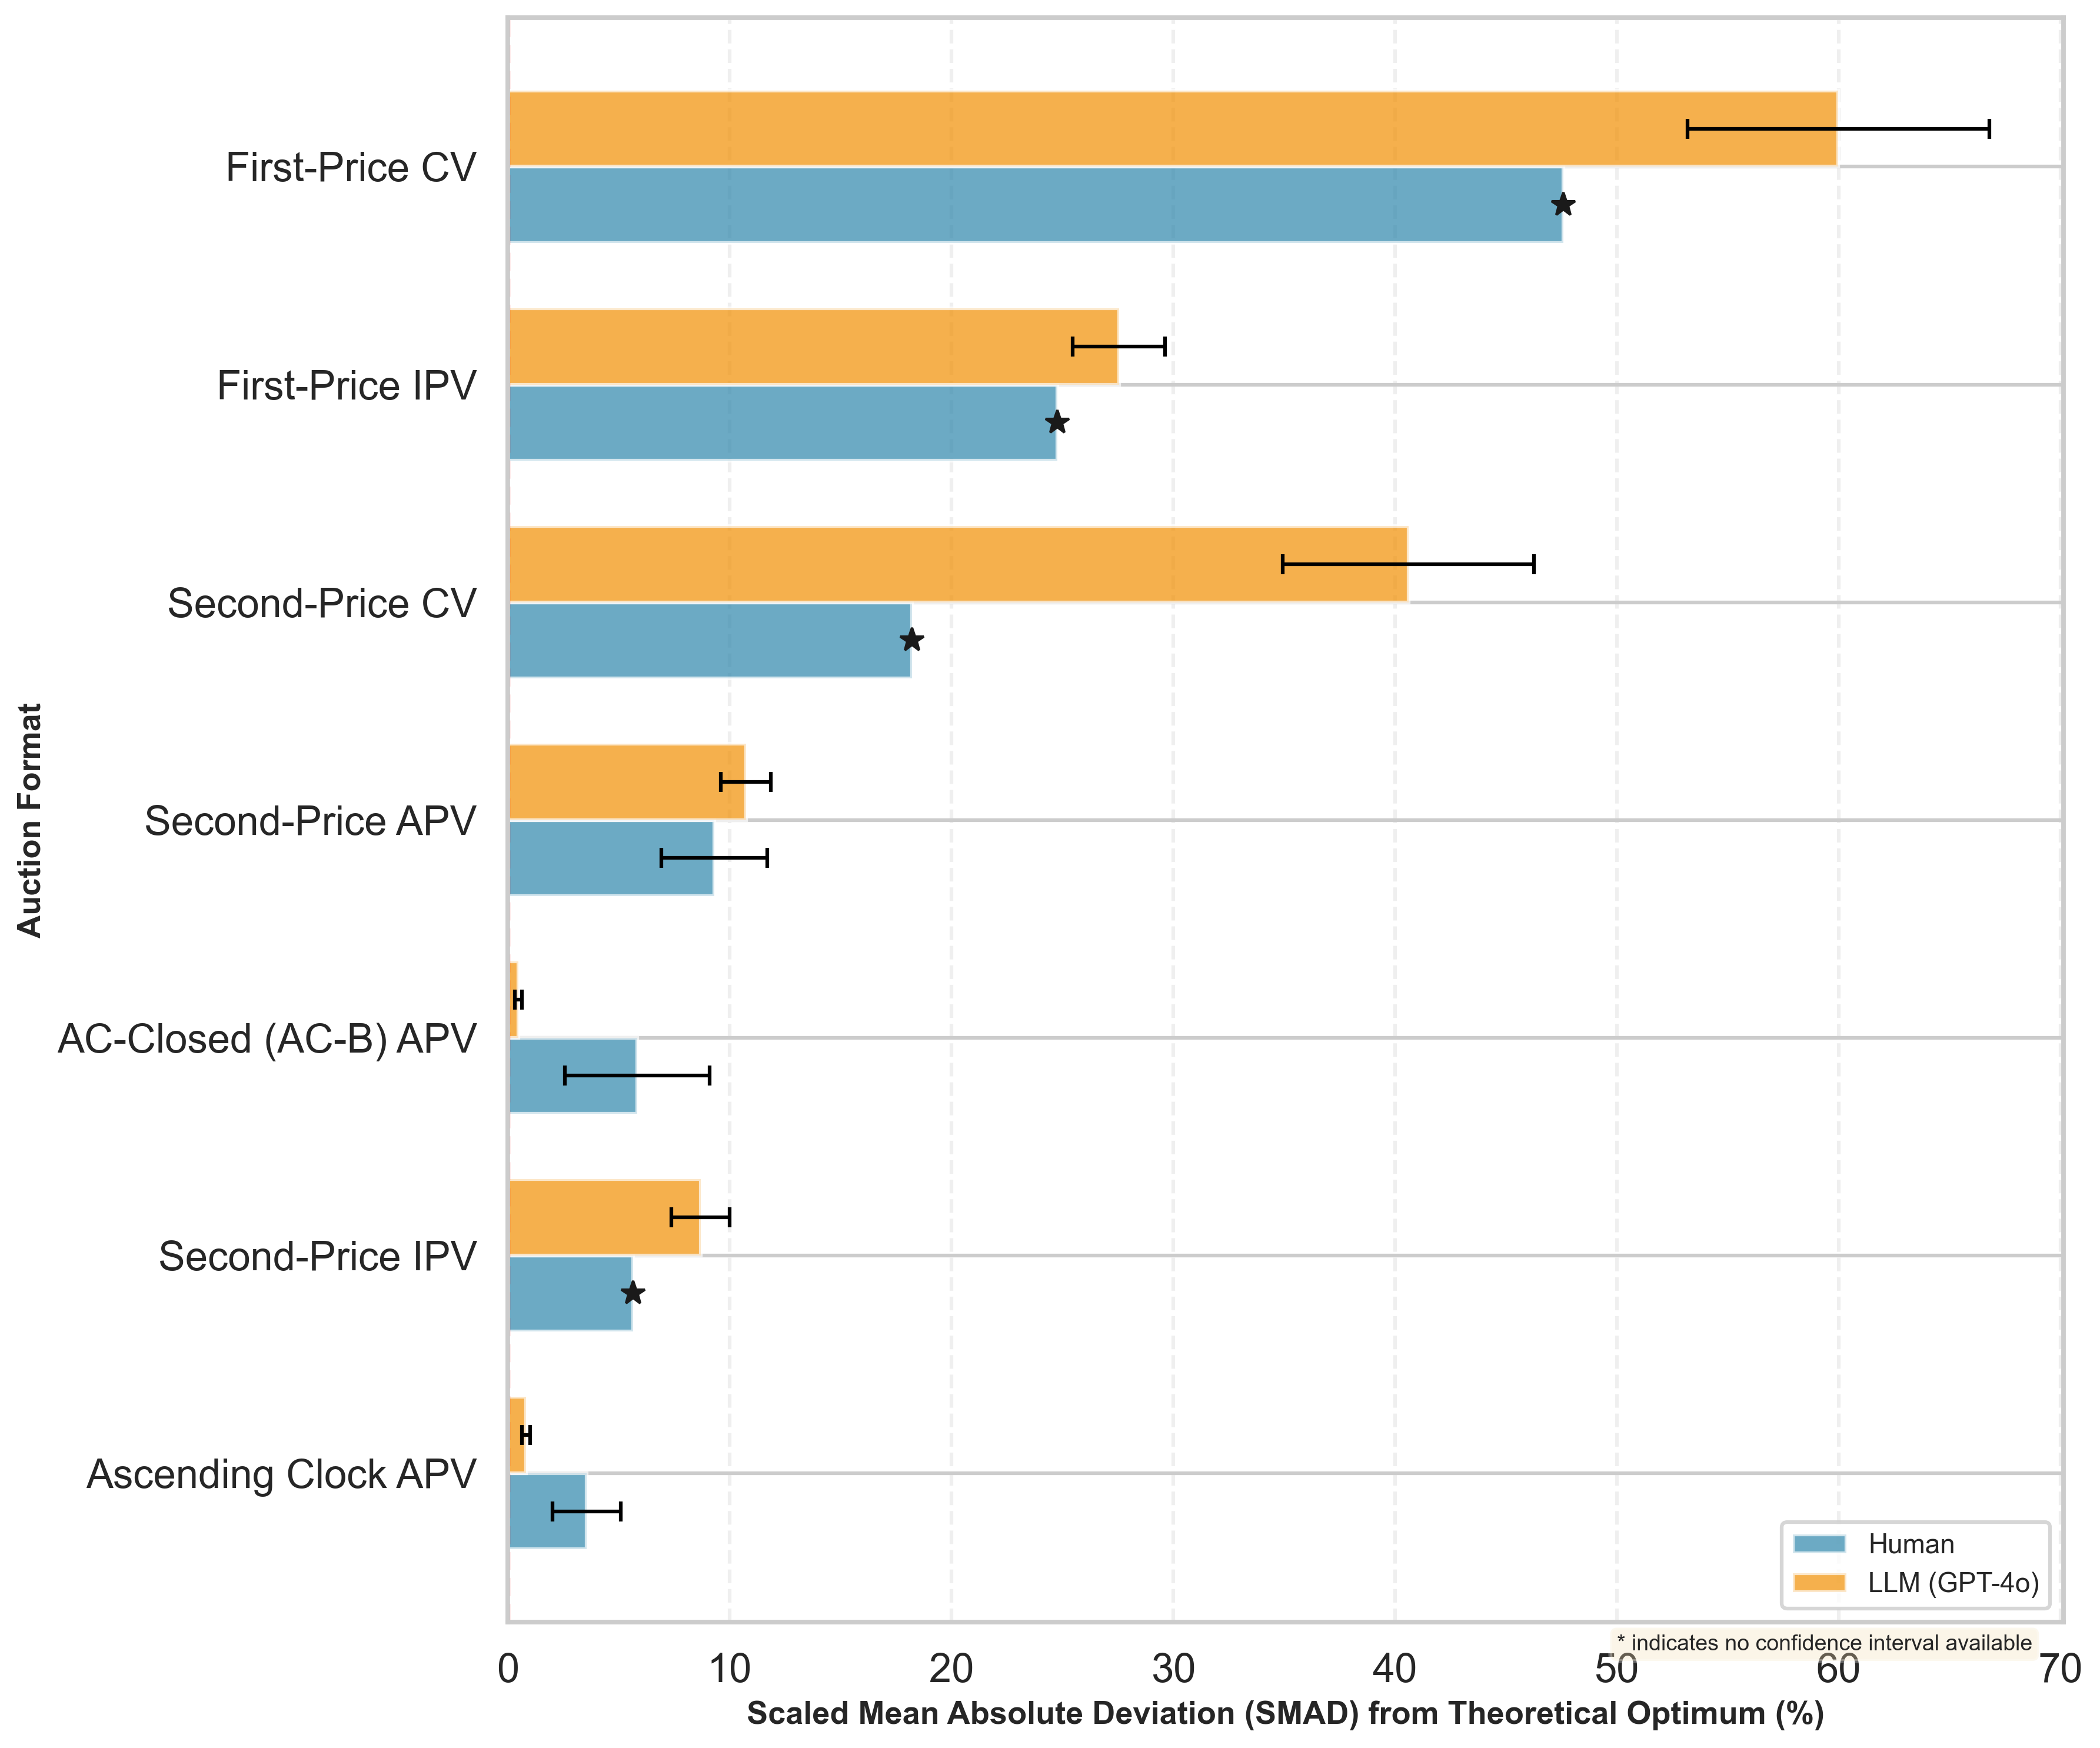
\includegraphics[scale=0.33]{figures/figure1.png}
    \caption{\textbf{Human vs LLM Bidding Behavior}: Blue bars stand for scaled mean absolute deviation (SMAD) between Human bidding and Theoretical Equilibrium. Yellow bars stand for SMAD between GPT-4o agents and Theoretical Equilibrium. Here, the LLM simulations are run with N=3 bidders.
    \label{fig:comparison}}
\end{figure}




\begin{figure}[h!]
    \centering
    
\includegraphics[scale=0.33]{figures/figure2_by_auction_type_10pct.png}
    \caption{Underbid vs Overbid After Removing Equal Bid ($\pm$2\% Threshold) Human vs LLM Across  Auction Types
    \label{fig:overbidding}}
\end{figure}


\subsection{LLM show difference in First-price and Second price Sealed-bid Auction}


We test whether LLM bidders adjust appropriately when the payment rule changes from first-price to second-price sealed-bid auctions, a particularly clean  economic environment because the allocation rule is unchanged, while the mapping from a bid to the winning payment differs sharply. 
In the IPV environment, Bayes--Nash equilibrium (BNE) predicts systematic bid shading in the first-price auction, whereas in the second-price auction truthful bidding is a dominant strategy. 

Figure~\ref{fig:comparison} summarizes overall deviations using SMAD (scaled mean absolute deviation from the theoretical benchmark). 
SMAD is substantially larger in first-price than second-price for both humans and GPT-4o (blue vs.\ yellow bars in Fig.~\ref{fig:comparison}). Concretely, human bidders exhibit FPSB SMAD of $24.76\%$ versus SPSB SMAD of $5.65\%$ (a $4.4\times$ difficulty gap), while GPT-4o shows FPSB SMAD of $27.55\%$ versus SPSB SMAD of $8.69\%$ (a $3.2\times$ gap). 
The fact that GPT-4o reproduces the qualitative ranking (FPSB harder than SPSB) suggests that it is sensitive to the additional strategic complexity introduced by paying one’s own bid.

However, the bid \emph{distributions} reveal sharp human--LLM divergences that are not visible from aggregate deviation magnitudes alone. Figure~\ref{fig:overbidding} decomposes errors directionally into underbidding vs.\ overbidding after removing near-optimal bids (within a $\pm2\%$ threshold) In the first-price IPV setting, both humans and GPT-4o primarily \emph{overbid} relative to the equilibrium benchmark, but GPT-4o’s overbidding is far more extreme: humans overbid $56.5\%$ of the time (underbid $43.5\%$) with a nontrivial mass of near-equilibrium bids removed ($10.4\%$), whereas GPT-4o overbids $85.9\%$ of the time (underbid $14.1\%$) and almost never lands near the benchmark ($0.7\%$ removed). This pattern is consistent with systematically more aggressive competition by LLM bidders in FPSB \citep{cox1988theory}.

In contrast, the second-price IPV setting flips direction. Human bidders are overwhelmingly on the overbidding side (overbid $96.0\%$, underbid $4.0\%$), consistent with the classic right-skewed bid distributions documented in Kagel and Levin (1993), where most bidding mass lies above value.\footnote{In an SPSB auction with $5$ players, \citet{kagel1993independent} observed that the distribution of bids was right-skewed, with the majority of the bidding mass (67\%) representing over-bidding relative to private values. However, this figure appears inconsistent with their reported regression of bids on values; specifically, both the intercept and the coefficient exceed 1, which would typically imply a more pervasive pattern of over-bidding than the percentage suggests.} GPT-4o, by contrast, produces a predominantly \emph{left-skewed} distribution with most mass on underbidding (underbid $81.3\%$, overbid $18.7\%$), despite truthful bidding being a dominant strategy. Notably, GPT-4o also places substantial probability mass near value (equal/near-equal bids removed: $29.2\%$), aligning with the fact that a sizable fraction of LLM bids exactly equal value in our runs.



\subsection{LLMs bid more truthfully in OSP auctions under affiliated private values}\label{session:OSP}


Beside the payment rules, another important variation in the economic environment  relates to the {\em interaction structure}, i.e., whether it is a one-shot sealed-bid auction or an iterative bidding process in a clock style. 
Clock auctions are dynamic formats where the price increases incrementally and bidders decide whether to stay in or drop out at each price point. 
For second-price auctions, although the sealed-bid format and the ascending-clock format share the same dominant strategy, human participants behave quite differently. 
A robust pattern in the experimental literature is that bidders do much better in clock-style auctions than in sealed-bid auctions. \citet{li2017obviously} provides an argument as to why clock auctions may be easier to recognize as strategy-proof for humans, and formalizes this as an equilibrium refinement on strategy-proofness called {\em obvious strategy-proofness (OSP)}. 
\citet{breitmoser2022obviousness} provide additional evidence that clock auctions improve truthful play, and also provide evidence that play under AC is slightly better than under AC-B. 


\textbf{Theoretical benchmarks and human baselines.}
We focus on an affiliated private values (APV) environment. While affiliation could in principle change incentives through correlation in values, the three auction formats we consider here are strategically equivalent: for the second-price sealed-bid (SP), the open ascending clock (AC), and the closed-information clock (AC-B), it remains a dominant strategy to bid (or drop out at) one’s value. Figure~\ref{fig:comparison} shows that human bidders deviate substantially less from truthful bidding in clock formats than in the sealed-bid SP benchmark: SMAD is $3.54\%$ in AC and $5.83\%$ in AC-B, compared to $9.31\%$ in SP. This ranking reinforces the standard interpretation that dynamic, incremental ``stay/exit'' decisions lower cognitive load relative to mapping a value into a single, one-shot bid.


\textbf{LLM results: a larger clock advantage, but not in sealed-bid Second Price.}
For GPT-4o agents, the clock advantage is even more pronounced. In the APV clock auctions, GPT-4o achieves near-truthful play: SMAD falls to $0.81\%$ in AC and $0.47\%$ in AC-B (a $77\%$--$92\%$ reduction relative to the human baselines). 
In contrast, in sealed-bid SP, GPT-4o remains at $10.73\%$ SMAD—close to the human level ($9.31\%$). 
Taken together, Figure~\ref{fig:comparison} suggests that GPT-4o is highly responsive to the interaction structure of the mechanism: breaking the decision into a sequence of simple threshold choices (``stay iff price is below value'') yields an order-of-magnitude improvement relative to the one-shot sealed-bid interface, even though the dominant-strategy benchmark is the same.

\textbf{Direction of mistakes: similar SMAD can mask qualitatively different behavior.}
To understand how these deviations arise, Figure~\ref{fig:overbidding} decomposes bidding errors by direction using a $\pm 2\%$ tolerance band around value (dropping near-equal bids and classifying the remainder as under- vs.\ over-bids). Despite similar aggregate deviation in SP-APV (SMAD $\approx 2\%$ for both humans and GPT-4o), the nature of the deviations differs strikingly: human bids are predominantly \emph{above} value (64.7\% overbidding vs.\ 35.3\% underbidding), while GPT-4o bids are predominantly \emph{below} value (92.4\% underbidding vs.\ 7.6\% overbidding). Thus, ``how far'' bidders deviate can look similar while ``which way'' they deviate is reversed—consistent with humans exhibiting competitive overbidding even under an incentive-compatible rule, while GPT-4o behaves overly conservatively in the sealed-bid interface.
In contrast, clock auctions substantially align both the magnitude and the \emph{shape} of behavior. In AC, humans and GPT-4o display an almost perfectly symmetric under/over split (49.2/50.8 vs.\ 50/50), but GPT-4o concentrates far more mass near truthful bidding (71.7\% within $\pm 2\%$ vs.\ 26.8\% for humans).


\subsection{LLM exhibits the Winner's Curse in Common-Value Auctions}
\label{sec:winners_curse}

Common-value auctions provide a particularly sharp test of whether bidders correctly condition on the adverse selection implicit in winning. In the canonical experimental design of \citet{kagel1986winner}, each bidder observes a noisy private signal $x$ about a common underlying value $x_0$. Winning is therefore ``bad news'': conditional on having the highest signal among $n$ bidders, the expected common value is strictly below $x$, with the gap widening in $n$.\footnote{In the standard symmetric-information design, $\mathbb{E}[x_0 \mid X=x_{1:n}] = x - \frac{n-1}{n+1}\varepsilon$ for signals away from boundary regions, where $\varepsilon$ controls signal noise. This highlights why competition exacerbates adverse selection: as $n$ rises, the winner must make a larger downward correction.} If bidders neglect (or incompletely correct for) this conditioning, they overbid relative to $\mathbb{E}[x_0\mid \text{win}]$ and the winner earns negative profits---the classic \emph{winner's curse}. Laboratory evidence documents both comparative statics emphasized in our setting: (i) winner losses become larger as the number of bidders increases, and (ii) institutions that reveal more information during the price discovery process attenuate the curse relative to sealed-bid first-price formats. For example, \citet{kagel1986winner} reports substantial negative profits conditional on winning that are markedly worse with more bidders (e.g., approximately $-\$1.68$ with $n=4$ versus $-\$3.68$ with $n=7$ in their benchmark conditions), and related work shows that the revenue advantage of ascending formats hinges on whether bidders have learned to avoid severe winner's-curse mistakes \citep{levin1996revenue}.


We evaluate whether LLM bidders exhibit analogous winner's-curse patterns in common-value \emph{first-price sealed-bid} (FPSB) auctions. Table~\ref{tab:winner_curse_llm} summarizes \emph{winner profits} in our simulations as we vary the number of bidders from 4 to 7 (holding the environment fixed). A clear winner’s-curse pattern emerges: winners lose money on average in every FPSB setting, and losses grow with competition (mean winner profit: $-2.54$ with 4 bidders, $-4.40$ with 5 bidders, $-5.46$ with 6 bidders, and $-5.55$ with 7 bidders). Consistent with this monotonic decline, the share of winners earning positive profits collapses from 24\% (4 bidders) to 0\% (7 bidders). One-sided tests strongly reject the hypothesis that winner profit is nonnegative in all FPSB treatments, confirming that LLM bidders fall prey to the winner’s curse\citep{kagel1986winner}.

To benchmark the role of auction format, we also simulate a common-value \emph{second-price sealed-bid} (SPSB) environment under the same information structure. The same comparative-static forces appear, but the curse is attenuated: with 4 bidders, winners earn positive profits on average (mean $=1.30$), profits are near zero with 5 bidders, and winner losses become statistically significant only once competition is sufficiently intense ($n\ge 6$). Thus, while both formats exhibit adverse-selection pressures that grow in $n$, LLM behavior displays a substantially stronger winner’s curse in FPSB than in SPSB, mirroring the qualitative ranking emphasized by the experimental literature\citep{levin1996revenue}.

\begin{table}[H]
\centering
\begin{tabular}{lccccc}
\toprule
\textbf{Auction} & \textbf{Bidders} & \textbf{Mean (Std.)} & \textbf{Median} & \textbf{\% Positive} & \textbf{$p$ (Profit $<0$)} \\
\midrule
FPSB & 4 & $-2.54$ (3.87) & $-3.00$ & 24.0\% & $<0.001^{***}$ \\
FPSB & 5 & $-4.40$ (3.63) & $-4.00$ & 6.0\%  & $<0.001^{***}$ \\
FPSB & 6 & $-5.46$ (3.82) & $-5.05$ & 4.0\%  & $<0.001^{***}$ \\
FPSB & 7 & $-5.55$ (2.93) & $-5.30$ & 0.0\%  & $<0.001^{***}$ \\
\midrule
SPSB & 4 & $1.30$ (4.87)  & $1.00$  & 58.0\% & 0.967 \\
SPSB & 5 & $0.07$ (4.35)  & $0.00$  & 46.0\% & 0.542 \\
SPSB & 6 & $-2.82$ (3.50) & $-1.75$ & 18.0\% & $<0.001^{***}$ \\
SPSB & 7 & $-2.83$ (2.78) & $-2.00$ & 12.0\% & $<0.001^{***}$ \\
\bottomrule
\end{tabular}
\caption{Winner profit in common-value auctions with LLM bidders. The last column reports one-sided $p$-values for the hypothesis that winner profit is negative. *** denotes $p < 0.001$.}
\label{tab:winner_curse_llm}
\end{table}



\subsection{LLMs respond to Interventions in Sealed-bid Auctions Differently}\label{session:Intervention}

Recent  studies consider whether behavior in strategy-proof auctions depends on how the mechanism is \emph{presented}, holding the underlying incentives fixed. In particular, \citet{gonczarowski2023strategyproofness} propose an \textit{extensive-form menu} description that compresses the dominant-strategy logic of a second-price sealed-bid (SPSB) auction into a short, one-sentence menu intended to make strategy-proofness salient. However, in their laboratory experiments this menu-framing does not meaningfully change human bidding relative to the traditional SPSB description, which they interpret as evidence that classic SPSB instructions may already be highly transparent. 
In contrast, \citet{breitmoser2022obviousness} show that \emph{reframing} SPSB as a dynamic ascending clock can substantially increase truth-telling, consistent with the idea that step-by-step ``stay/exit'' choices reduce the cognitive burden of mapping a value into a single sealed bid.

Figure~\ref{fig:intervention} reports the same two interventions evaluated on LLM bidders. Across all conditions, we summarize behavior using the distribution of \emph{scaled deviations} $(b-v)$ \footnote{We used the same scaling factor as in the definition of SMAD in Sec~\ref{sec:method}} (where negative values correspond to underbidding relative to truthful play, and positive values to overbidding). 
Under the traditional SPSB framing, LLM bids are systematically below value on average (mean $=-0.106$), with substantial dispersion (std.\ $=0.099$). The menu-framing intervention does not materially change this pattern: the distribution remains centered on underbidding (mean $=-0.143$) and is, if anything, more dispersed (std.\ $=0.166$). Consistent with the visual overlap in the left panel, we fail to detect a robust distributional shift under a nonparametric Mann--Whitney test ($p=0.228$). While a Welch $t$-test rejects equality of means at conventional levels ($p=0.017$), the effect size is small (Cohen's $d=0.27$), suggesting that any change induced by menu-framing is modest and not stable across tests, consistent with the findings in \citet{gonczarowski2023strategyproofness}.

By contrast, the clock-framing intervention produces a sharp and unambiguous change in LLM bidding. As shown in the right panel of Figure~\ref{fig:intervention}, clock-framing shifts the distribution substantially toward truthful play, with the mean deviation moving from $-0.106$ to $-0.019$ ( $\approx 82\%$ reduction in average underbidding) and the dispersion collapsing from $0.099$ to $0.024$ (about a four-fold reduction). This shift is highly significant under both Mann--Whitney and Welch tests (both $p<0.001$) and large in magnitude (Cohen's $d=-1.21$). This suggests that LLM bidders respond strongly to an intervention that changes the \emph{clock  framing} of the same dominant-strategy mechanism, consistent with the findings in \citet{breitmoser2022obviousness}.





%
\begin{figure}[h!]
    \centering
    
\includegraphics[width=0.9\linewidth]{figures/figure3_intervention_comparison.png}
    \caption{Effects of menu-framing and clock-framing on LLM bidding deviations in second-price auctions. Menu-framing yields no detectable distributional shift, whereas clock-framing sharply increases truth-telling. Only LLM simulation data are shown.} 
    \label{fig:intervention}
\end{figure}